\documentclass[12pt,a4paper]{article}
\usepackage[utf8x]{inputenc}
\usepackage{ucs}
\usepackage[english,russian]{babel}
\usepackage[OT1]{fontenc}
\usepackage{amsmath}
\usepackage{amsfonts}
\usepackage{amssymb}
\usepackage{wasysym}
\usepackage{physics}
\usepackage{wrapfig}

\usepackage[left=2cm,right=2cm,top=2cm,bottom=2cm,includefoot,footskip=1.5cm]{geometry}

\usepackage{fancyhdr}
\pagestyle{fancy}

\usepackage[T1]{fontenc}
 
\usepackage{indentfirst}
%% Sets page size and margins
\usepackage[dvips]{graphicx}
\graphicspath{{noiseimages/}}
\usepackage[colorinlistoftodos]{todonotes}
\usepackage[colorlinks=true, allcolors=blue]{hyperref}

\rhead{\small Д.\,Павлов, А.\,Савко, МФТИ}
\lhead{Лабораторная работа №3.2.1}

\author{Дмитрий Павлов, 790 \\  Александр Савко, 790}
\title {\textbf{Сдвиг фаз в цепи переменного тока}}

\begin{document}
\maketitle
\newpage
\tableofcontents 

\newpage

\section{Вступление.}
    \subsection{Цель работы.}
        Исследование зависимости сдвига фаз между током и напряжением от сопротивления в $RC$- и в $RL-$цепи; определение добротности колебательного контура, при помощи полученной в работе зависимости сдвига фаз от частоты вблизи резонанса; оценка диапазона работы фазовращателя.
        
    \subsection{Оборудование.}
        \begin{itemize}
            \item Звуковой генератор (ЗГ);
            \item Двухканальный электронный осциллограф (ЭО);
            \item Магазин емкостей;
            \item Магазин сопротивлений;
            \item Эталонная катушка индуктивности;
            \item Резисторы;
            \item Мост переменного тока.
        \end{itemize}

    \subsection{Экспериментальная установка.}
         \begin{wrapfigure}{2}{0.6\linewidth}
        	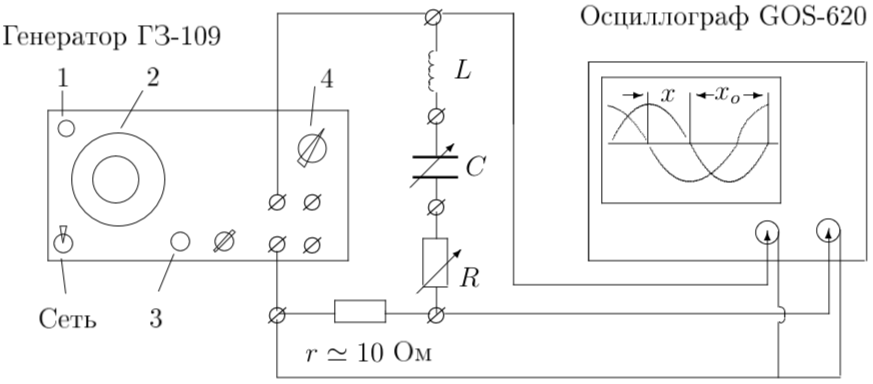
\includegraphics[width=\linewidth]{ris1.png}
        	\hspace{44pt}{Рисунок 1 -- Схема для исследования сдвига фаз между током и напряжением в цепи переменного тока.}
        	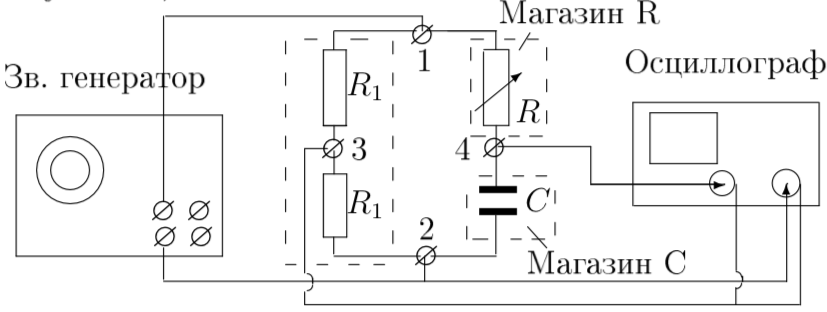
\includegraphics[width=\linewidth]{ris2.png}
        	\hspace{44pt}{Рисунок 2 -- Схема фазовращателя.}
        \end{wrapfigure}
        
        Схема для исследования сдвига фаз между током и напряжением в цепи переменного тока представлена на рис. 1. Эталонная катушка $L$, магазин емкостей $C$ и магазин сопротивлений $R$ соединены последовательно и через дополнительное сопротивление $r$ подключены к источнику синусоидального напряжения - звуковому генератору.
        
        Сигнал, пропорциональный току, снимается с сопротивления $r$, пропорциональный напряжению - с генератора. Оба сигнала подаются на универсальный осциллограф. Этот осциллограф имеет два канала вертикального отклонения, что позволяет одновременно наблюдать на экране два сигнала.
        
        Схема фазовращателя, изображенная на рис. 2, содержит два одинаковых резистора $R_1$, смонтированных на отдельной плате, магазин сопротивлений $R$ и магазин емкостей $C$.

\newpage
\section{Основная работа.}
    \subsection{Исследование зависимости сдвига фаз между током и напряжением от $R$ в $RC-$цепи}
        Пользуясь схемой, изображенной на рис. 1, найдем зависимость сдвига фаз между током и напряжением от $R$ в $RC-$цепи. Для этого закоротим катушку индуктивности. На магазине емкости поставим емкость $C = 0.5$ мкФ, $\nu = 1$ кГц.
        
        Рассчитаем реактивное сопротивление цепи по формуле: $X_1 = 1/(\Omega C) = 1/(2 \pi \nu C)$. Где $\Omega = 2 \pi \nu$ - циклическая частота.
        
        \[
        X_1 = \frac{1}{\Omega C} = \frac{1}{2 \pi \nu C} = \frac{1}{2 \pi \cdot 1000 \text{Гц} \cdot 0.5 \text{мкФ}} = 318.3 \text{Ом}
        \]
        
        Увеличивая сопротивление $R$ от нуля до $10 \cdot X_1$, проведем измерения сдвига фаз $\psi$.
        
        \begin{table}[!h]
        \begin{flushleft}
       		\hspace{80}\textbf{Таблица 1} -- Сдвиг фаз в $RC-$контуре в зависимости от  $R$.\\
        \end{flushleft}
            \begin{center}
                \begin{tabular}{ | l | l | l | l |}
                    \hline
                    $R$, Ом &   $x$, см &  $x_0$, см &   $\psi$  \\
                    \hline
                    0   &   2.5 &   5   &   0.5$\pi$\\
                    200 &   1.6 &   5   &   0.32$\pi$\\
                    400 &   1.2 &   4.4 &   0.245$\pi$\\
                    600 &   0.4 &   4.5 &   0.089$\pi$\\
                    900 &   0.6 &   5   &   0.12$\pi$\\
                    1200&   0.2 &   4.5 &   0.083$\pi$\\
                    \hline                
                \end{tabular}
            \end{center}
        \end{table}
            
    \subsection{Исследование зависимости сдвига фаз между током и напряжением от $R$ в $RL-$цепи}
        Пользуясь схемой, изображенной на рис. 1, найдем зависимость сдвига фаз между током и напряжением от $R$ в $RL-$цепи. Для этого закоротим магазин емкостей. На катушке поставим индуктивность $L = 50$ мГн, $\nu = 1$ кГц.
        
        Рассчитаем реактивное сопротивление цепи по формуле: $X_2 = \Omega L = 2 \pi \nu C$. 
        
        \[
        X_2 = \Omega L = 2 \pi \nu L = 2 \pi \cdot 1000 \text{Гц}\cdot 50\text{Гн} = 314 \text{Ом}
        \]
        
        Увеличивая сопротивление $R$ от нуля до $10 \cdot X_2$, проведем измерения сдвига фаз $\psi$.
        
        \begin{table}[!h]
        \begin{flushleft}
       		\hspace{80}\textbf{Таблица 2} -- Сдвиг фаз в $RL-$контуре в зависимости от  $R$.\\
        \end{flushleft}
            \begin{center}
                \begin{tabular}{ | l | l | l | l |}
                    \hline
                    $R$, Ом &   $x$, см &  $x_0$, см&   $\psi$      \\
                    \hline
                    0       &   2.2     &   4.9     &   0.45$\pi$   \\
                    200     &   1.4     &   4.9     &   0.29$\pi$   \\
                    600     &   0.6     &   4.9     &   0.12$\pi$   \\
                    900     &   0.4     &   4.9     &   0.082$\pi$  \\
                    1200    &   0.2     &   4.9     &   0.041$\pi$  \\
                    \hline                
                \end{tabular}
            \end{center}
        \end{table}
        
    \subsection{Исследование зависимости сдвига фаз между током и напряжением от частоты в $RLC$-контуре}
        В цепи, изображенной на рис. 1, Установим значения $R = 0$, $L = 50$ мГн, $C = 0.5$ мкФ. Рассчитаем резонансную частоту по формуле: $\nu = 1/(2 \pi \sqrt{LC})$.
        
        \[
        \nu = \frac{1}{(2 \pi \sqrt{LC})} = \frac{1}{2 \pi \sqrt{50\text{мГн} \cdot 0.5 \text{мкФ}}} = 1006 \text{Гц}
        \]
        
        Снимем зависимость сдвига фаз от частоты. Для этого:
        \begin{itemize}
            \item Подберем частоту ЗГ, чтобы получить резонанс в цепи. При резонансе $\psi = 0$, и нулевые значения двух синусоид должны совместиться, а при равенстве амплитуд синусоиды полностью совпадают.
            
            \[
            \nu_{\text{эксп}} = 1020 \text{Гц}.
            \]
            \item Оценим по картинке на экране ЭО диапазон измерения частоты, в котором сдвиг фазы меняется от $\pi/3$ до $-\pi/3$.
            \item Снимем зависимость сдвига фаз от частоты в этом диапазоне, меняя частоту в обе стороны от резонансного значения. С изменением частоты меняется расстояние $x_0$, которое занимает половина периода синусоиды, поэтому каждый раз фиксируем отношение $x/x_0$.
            
            \begin{table}[!h]
            \begin{flushleft}
           		\hspace{20}\textbf{Таблица 3} -- Сдвиг фаз в $RLC-$контуре в зависимости от частоты при $R = 0$ Ом.\\
            \end{flushleft}
                \begin{center}
                    \begin{tabular}{ | l | l | l | l | l | l | l | l |}
                        \hline
                        $\nu$, Гц   &   $x$, см &  $x_0$, см&   $\psi$  &   $\nu$, Гц   &   $x$, см &  $x_0$, см&   $\psi$  \\
                        \hline
                        910         &   1.6     &   5.3     &           &   1000        &   0.3     &   4.8     &      \\
                        930         &   1.5     &   5       &           &   1040        &   0.5     &   4.8     &      \\
                        950         &   1.2     &   5       &           &   1060        &   0.8     &   4.7     &   \\
                        970         &   0.9     &   5       &           &   1090        &   1       &   4.6     &      \\
                        990         &   0.6     &   5       &           &   1100        &   1.2     &   4.5     &    \\
                        1020        &   0       &   4.8     &           &   1120        &   1.3     &   4.4     &    \\
                        \hline         
                    \end{tabular}
                \end{center}
            \end{table}   
            \item Повторим измерения сдвига фаз для сопротивления $R = 100$ Ом.
            
            \begin{table}[!h]
            \begin{flushleft}
           		\hspace{20}\textbf{Таблица 4} --  Сдвиг фаз в $RLC-$контуре в зависимости от частоты при $R = 100$ Ом.\\
            \end{flushleft}
                \begin{center}
                    \begin{tabular}{ | l | l | l | l | l | l | l | l |}
                        \hline
                        $\nu$, Гц   &   $x$, см &  $x_0$, см&   $\psi$  &   $\nu$, Гц   &   $x$, см &  $x_0$, см    &   $\psi$  \\
                        \hline
                        900         &   0.8     &   5.2     &           &   1020        &   0       &   4.8         &      \\
                        920         &   0.6     &   5       &           &   1040        &   0.2     &   4.8         &      \\
                        940         &   0.4     &   5       &           &   1060        &   0.4     &   4.7         &      \\
                        960         &   0.3     &   5       &           &   1090        &   0.5     &   4.6         &      \\
                        980         &   0.2     &   4.9     &           &   1100        &   0.6     &   4.5         &    \\
                        1000        &   0       &   4.8     &           &   1120        &   0.6     &   4.5         &    \\
                        \hline         
                    \end{tabular}
                \end{center}
            \end{table}
        \end{itemize}
        
    \subsection{Проверка приборов с помощью моста E7-8}
        \begin{center}
            \begin{tabular}{ | l | l | l |}
                \hline
                Значение        &   Номинальное, Ом &   Реальное, Ом \\
                \hline
                r               &   12.4            &   12.43    \\
                $R_\text{кат}$  &   31.5            &   32.77    \\
                \hline                
            \end{tabular}
        \end{center}
        
    \subsection{Исследование работы фазовращателя}
        Необходимо найти сопротивление $R$, при котором сдвиг фаз равен $\pi/2$. Соберем схему, изображенную на рис. 2, и установим $C = 0.5$мкФ, $\nu = 1$ кГц. При $R = 3800$ Ом сдвиг фаз равен $\pi/2$.
        
\newpage
\section{Проведение эксперимента.}

       
       
        \begin{table}[!h]
        \begin{flushleft}
       		\hspace{134}\textbf{Таблица 1} -- Параметры шариков\\
        \end{flushleft}
            \begin{center}
                \begin{tabular}{ | l | l | l | l |}
                \hline
                Номер шарика            &   1       &   2       &   3       \\
                \hline
                Обхват лентой, см       &   64      &   84      &   66      \\
                Радиус, см              &   10,19   &   13,37   &   10,5    \\
                Образующая конуса, см   &   17,6    &   27      &   18,2   \\
                Высота конуса, см       &   14,4    &   24,4    &   14,8    \\
                Площадь шарика, см$^2$  &   1216    &   2257    &   1292    \\
                Толщина, мм             &   0,0123  &   0,00664 &   0,0116  \\  
                \hline
                \end{tabular}   
            \end{center}
        \end{table}
       

        Радиус вычислен из значения обхвата ленты по формуле: $R = \frac{L}{2\pi}$
        
        Высота конуса найдена по теореме Пифагора из значений радиуса и образующей:
        
        $h = \sqrt{l^2 - R^2}$
        
        Площадь $S = \frac{1}{2}(\pi d^2 + \pi ld)$, где $d$ - диаметр шарика, $l$ - образующая конуса
        
        Толщина найдена по формуле $\delta = \frac{m}{S \cdot \rho}$


  
    \subsection{Коэффициент диффузии:}
        Коэффициент диффузии найдем с помощью закона Фика, для этого нужно экспериментально найти количество покидающих за секунду шарик молекул ($\Delta n$ и $\delta$ известны). Заметим что со временем шарик уменьшается в размерах, значит, из закона Архимеда $F = g \rho V$, должна меняться подъемная сила, действующая на шарик. Зависимость $F_{\text{арх}}(t)$ можно найти с помощью груза и весов, весы будут показывать силу давления груза, к которому привязан шарик.
        Со стороны шарика на груз действует изменяющаяся со временем сила. Изменение этой  силы можно представить как
        \[
        \Delta M(t) = \beta \cdot t = D S \frac{\rho_0 - \rho_{He}}{\delta} t,
        \]
        где $\beta$ - угол наклона графика $\Delta M(t)$. Его можно найти построив график  зависимости силы давления груза, к которому привязан шарик, от времени.
    \newpage
        \subsubsection{Найдем зависимость силы давления груза на весы от времени:}
        Проведем три серии измерений. В первой серии используем груз №1,  во втором -- груз №2, в третьем -- груз №1.
        \begin{table}[!h]
        \begin{flushleft}
       		\hspace{30}\textbf{Таблица 2} -- Показания весов, измеряющих массу груза, первое измерение \\
        \end{flushleft}
            \begin{center}
                \begin{tabular}{ | l | l | l | l | l | l | l | l | l | l |l | l | l | l | l | l | l | l | l | l |}
                \hline
                m, г    &  6,65    &   6,72    &   6,76    &   6,8 &   6,83    &   6,87     &  6.93    &   7,00    &   7,04    &   7,11    &  7,24     &  7,39 \\
                \hline
                t, мин    &  0       &   4       &   8       &   12  &   16,25   &   20       &   25     &   30      &   35      &   40      &  50       &   65  \\
                \hline                
                \end{tabular}
            \end{center}
        \end{table}
       
        \begin{table}[!h]
        \begin{flushleft}
       		\hspace{30}\textbf{Таблица 3} -- Показания весов, измеряющих массу груза, второе измерение \\
        \end{flushleft}
            \begin{center}
                \begin{tabular}{| l | l | l | l | l | l | l | l | l | l |l | l | l | l | l | l | l | l | l | l |}
                \hline
                 m, г    &  8,09    &   8,27    &   8,36    &   8,45    &   8,53    &   8,78     &   9,00    &  9,18    &   9,35    &   9,51    &   9,68    &  10,04 \\
                \hline
                t, мин    &  0       &   5       &   7,45    &   10      &   12      &   19.25   &   25      &    30     &   35      &   40      &   45      &  55    \\
                \hline                
                \end{tabular}
            \end{center}
        \end{table}
       
        \begin{table}[!h]
        \begin{flushleft}
       		\hspace{30}\textbf{Таблица 4} -- Показания весов, измеряющих массу груза, третье измерение \\
        \end{flushleft}
            \begin{center}
                \begin{tabular}{| l | l | l | l | l | l | l | l | l | l |l | l | l | l | l | l | l | l | l | l |}
                \hline
                m, г    &  8,82    &   8,86    &   8,36    &   8,92    &   8,96    &   9,00    &   9,04    &   9,1     &   9,15    &   9,23    &   9,29    &  9,34 \\
                \hline
                t, мин    &  0       &   4       &   8,5     &   12      &   16      &   20      &   26      &    30     &   35      &   40      &   45      &  50   \\
               \hline                
               \end{tabular}
            \end{center}
        \end{table}
        \begin{figure}[h!]
        	\begin{center}
        		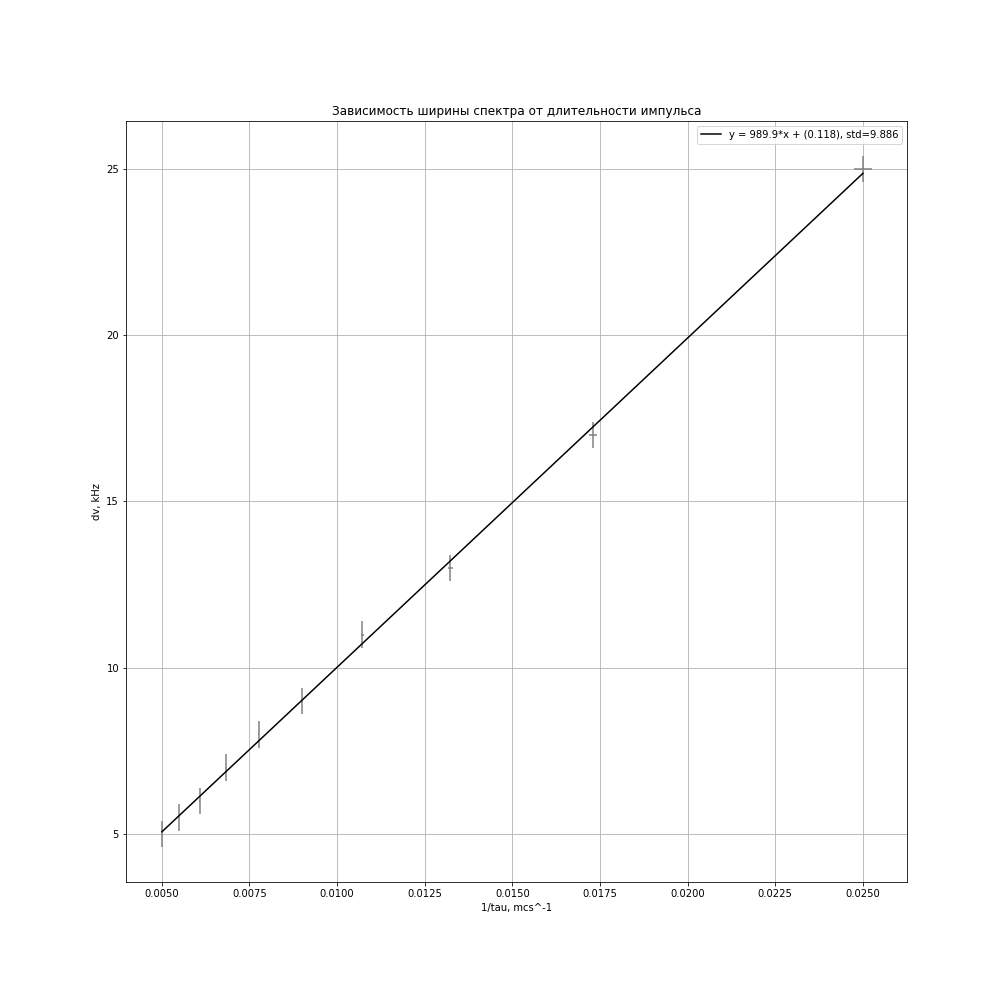
\includegraphics[width=0.9 \textwidth]{1}\\
            	{\scriptsize
            	\begin{center}
            	\hspace{69pt}{Рисунок 2 -- График зависимости массы шарика с грузом от времени в 1 измерении}
            	\end{center}}
        	\end{center}
            \label{scheme1}
        \end{figure}

        \begin{figure}[h!]
        	\begin{center}
        		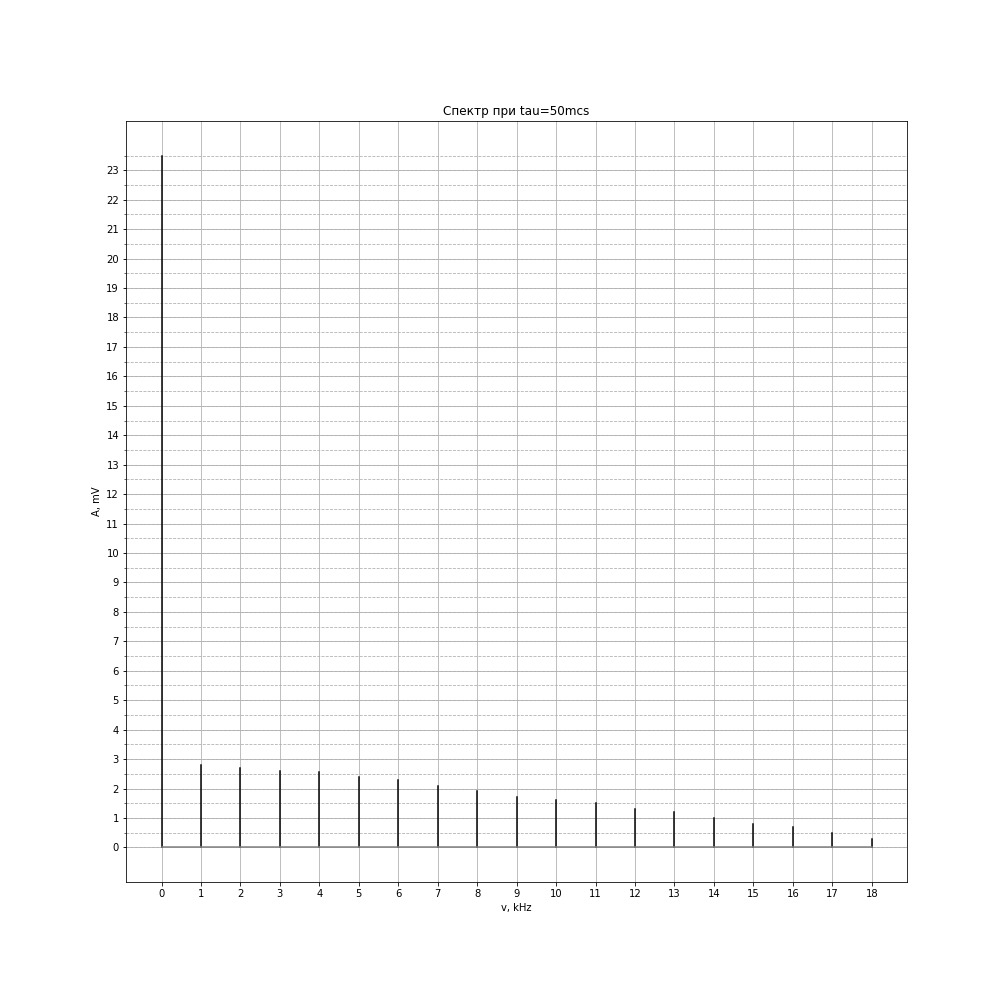
\includegraphics[width=0.9 \textwidth]{2}\\
            	{\scriptsize
            	\begin{center}
            	\hspace{69pt}{Рисунок 3 -- График зависимости массы шарика с грузом от времени в 2 измерении}
            	\end{center}}
        	\end{center}
            \label{scheme1}
        \end{figure}

        \begin{figure}[h!]
        	\begin{center}
        		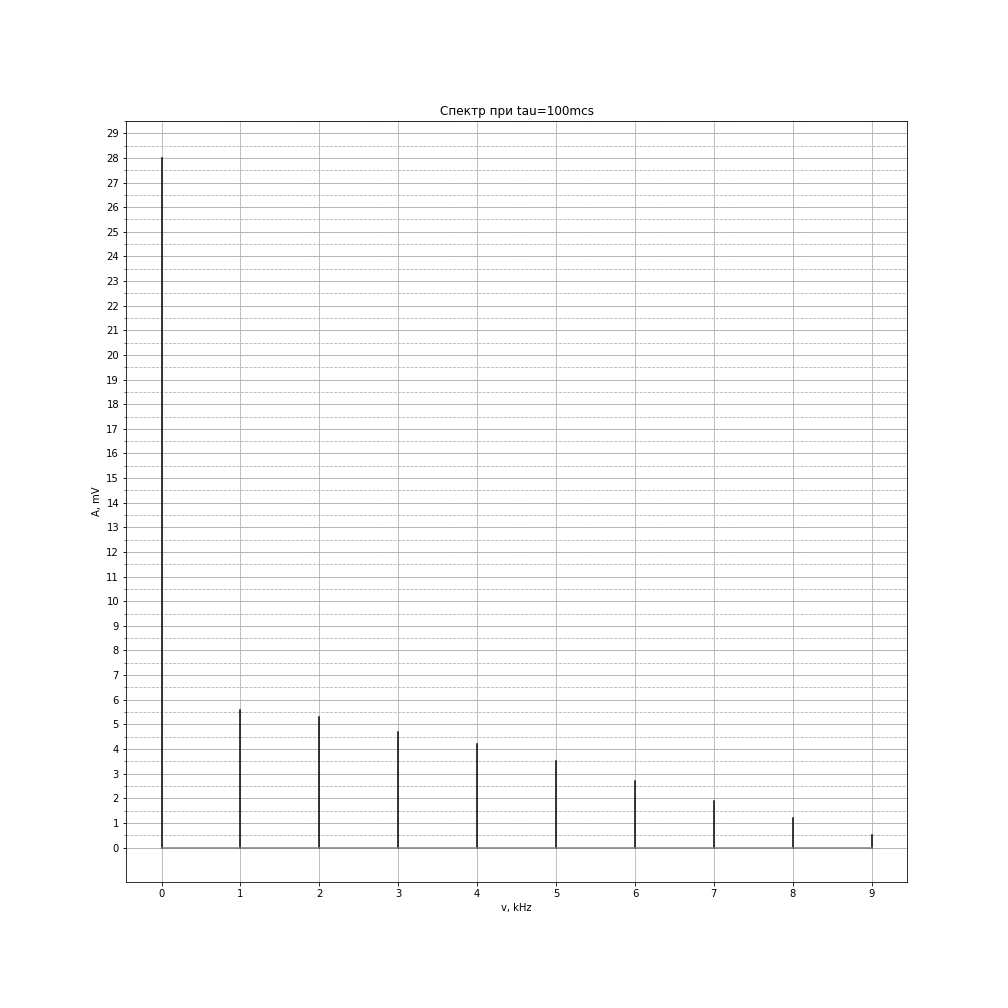
\includegraphics[width=0.9 \textwidth]{3}\\
            	{\scriptsize
            	\begin{center}
            	\hspace{69pt}{Рисунок 4 -- График зависимости массы шарика с грузом от времени в 3 измерении}
        	\end{center}}
        	\end{center}
            \label{scheme1}
        \end{figure}

        \begin{table}[!h]
        \begin{flushleft}
        Рассчитаем по МНК коэффициент наклона графиков. Полученные результаты представлены в таблице 5.\\
       		\hspace{140}\textbf{Таблица 5} -- Угол наклона графика \\
        \end{flushleft}
             \begin{center}
                \begin{tabular}{ | l | l |}
                \hline
                           &   Угол наклона $\beta$, г/мин\\
                \hline
                Шарик №1    &    0,0113      \\
                \hline
                Шарик №2    &    0,0351      \\
                \hline
                Шарик №3    &    0,0113      \\
                \hline
                \end{tabular}
            \end{center}
        \end{table}
       
        \newpage
        \subsubsection{Вычисление коэффициента диффузии}
        Воспользуемся соотношением:
            \[
            D = \frac{\beta \delta}{S(\rho_0 - \rho)},
            \]
        где толщина стенки $\delta = \frac{m_\text{об}}{S\rho_\text{рез}}$.\\        
       
        Получаем значения коэффициента диффузия: таблица 6.
       
        \begin{table}[!h]
        \begin{flushleft}
       		\hspace{10}\textbf{Таблица 6} -- Коэффициент диффузии для каждого шарика \\
        \end{flushleft}
            \begin{center}
                \begin{tabular}{ | l | l | l |  l |}
                \hline
                &   Площадь, см$^2$ &   Толщина стенок, мм  &   Коэффициент диффузии $10^{-7}$ $\frac{\text{см}^2}{\text{c}}$   \\
                \hline
                Шарик №1    &   1216,75   & 0,0123  &   1,91      \\
               \hline
                Шарик №2    &   2257,56   & 0,00664 &   1,74     \\
               \hline
                Шарик №3    &   1292,64   & 0,0116  &   1,69     \\
               \hline
               \end{tabular}
            \end{center}
        \end{table}
 
    \subsection{Погрешности измерений}
        \subsubsection{Погрешность углового коэффициента:}
       
            \begin{center}
                $\sigma_{k} = \frac{1}{\sqrt{n}}\sqrt{\frac{\langle y^2 \rangle - \langle y \rangle ^2}{\langle x^2 \rangle - \langle x \rangle ^2} - k^2}$
            \end{center}
               
            \begin{table}[!h]
            \begin{flushleft}
                \hspace{10}\textbf{Таблица 7} -- Расчет случайной погрешности по МНК \\
                \end{flushleft}
                    \begin{center}
                        \begin{tabular}{ | l | l | l | l | l | l | l | l | l |}
                        \hline
                        &   $\langle x^2 \rangle$ &   $\langle y^2 \rangle$  &   $\langle x \rangle ^2 $  &   $\langle y \rangle ^2$ &   $k$ &   $\sigma_k$, $10^{-4}$  &   $\varepsilon$ &  $\varepsilon$, \%   \\
                        \hline
                        Шарик №1    &   996,9218    & 48,2777   &   647,0664   &   48,2330  &   0,0113  &   0,66   &   0,0058  &   0,6  \\
                        \hline
                        Шарик №2    &    841,2554   & 80,2184   &  558,9284    &   79,8640  &   0,0354  &   4,4    &   0,012   &   1,2  \\
                        \hline
                        Шарик №3    &    817,8541   & 82,6447   &   570,0156   &   82,6129  &   0,0113  &   1,8    &   0,016   &   1,6 \\
                        \hline
                        \end{tabular}
                    \end{center}
                \end{table}    
    \newpage            
        \subsubsection{Погрешность вычисления коэффициента диффузии:}
            Коэффициент диффузии находим по формуле:
            \[
            D = \frac{\beta \delta}{S(\rho_0 - \rho)},
            \]
            где $\delta$ и $S$ находили по формулам:
            \begin{center}

            
            $\delta = \frac{m_\text{об}}{S \rho_\text{рез}}$    
            
            $S = \frac{1}{2}(\pi d^2 + \pi l d)$.    
            \end{center}

            
            \begin{table}[!h]
            \begin{flushleft}
                \hspace{10}\textbf{Таблица 8} -- Причины погрешности \\
                \end{flushleft}
                    \begin{center}
                        \begin{tabular}{ | l | l | l | l | l | l | l | l | l |}
                        \hline
                        Измерение           &   Значение    &   Абс. погрешность    &   Отн. погрешность   \\
                        \hline
                        Обхват лентой       &   64 см       &   0,5 мм              &   7,8 $\cdot$ $10^{-4}$\\
                        \hline
                                            &   84 см       &   0,5 мм              &   5,9 $\cdot$ $10^{-4}$\\
                        \hline
                                            &   66 см       &   0,5 мм              &   7,6 $\cdot$ $10^{-4}$\\
                        \hline
                        Образующая конуса   &   17,6 см     &   0,5 мм              &   2,8 $\cdot$ $10^{-3}$\\
                        \hline
                                            &   27 см       &   0,5 мм              &   1,8 $\cdot$ $10^{-3}$\\
                        \hline
                                            &   18,2 см     &   0,5 мм              &   2,7 $\cdot$ $10^{-3}$\\
                        \hline
                        \end{tabular}
                    \end{center}
                \end{table}  
                
            Погрешность измерения площади шарика:
            \[
            \sigma(S) = S \sqrt{2^2(\frac{\sigma(d)}{d})^2 + (\frac{\sigma(l)}{l})^2 + (\frac{\sigma(d)}{d})^2}
            \]
            
            \begin{table}[!h]
            \begin{flushleft}
                \hspace{10}\textbf{Таблица 9} -- Погрешность измерения площади \\
                \end{flushleft}
                    \begin{center}
                        \begin{tabular}{ | l | l | l | l | l | l | l | l | l |}
                        \hline
                                    &   Значение    &   Абс. погрешность    &   Отн. погрешность    &   Отн. погрешность,\% \\
                        \hline
                        Шарик № 1   & 1216,75 см$^2$&   4   см$^2$          &   0,003               &   0,3\%               \\
                        \hline
                        Шарик № 2   & 2257,56 см$^2$&  5   см$^2$          &   0,002               &   0,2\%               \\
                        \hline
                        Шарик № 3   & 1292,64 см$^2$&  4   см$^2$          &   0,003               &   0,3\%               \\
                        \hline
                        \end{tabular}
                    \end{center}
                \end{table}  
                
            Погрешность измерения толщины оболочки равна погрешности измерения площади:
            \[
            \frac{\sigma(\delta)}{\delta} = \frac{\sigma(S)}{S}.
            \]
            Тогда погрешность измерения диффузии:
            \[
            \sigma(D) = D \sqrt{(\frac{\sigma(\beta)}{\beta})^2 + (\frac{\sigma(\delta)}{\delta})^2 + (\frac{\sigma(S)}{S})^2}.
\]
            
            \begin{table}[!h]
            \begin{flushleft}
                \hspace{10}\textbf{Таблица 9} -- Погрешность измерения коэффициента диффузии \\
                \end{flushleft}
                    \begin{center}
                        \begin{tabular}{ | l | l | l | l | l | l | l | l | l |}
                        \hline
                                    &   Значение    &   Абс. погрешность   &   Отн. погрешность    &   Отн. погрешность \\
                        \hline
                        Шарик № 1   &   1,91 $\cdot$ $10^{-7}$ $\frac{\text{см}^2}{\text{c}}$   &   1,34 $\cdot$ $10^{-9}$ $\frac{\text{см}^2}{\text{c}}$   &   0,007   &   0,7\%               \\
                        \hline
                        Шарик № 2   &   1,74 $\cdot$ $10^{-7}$ $\frac{\text{см}^2}{\text{c}}$   &   2,09 $\cdot$ $10^{-9}$ $\frac{\text{см}^2}{\text{c}}$   &   0,012   &   1,2\%               \\
                        \hline
                        Шарик № 3   &   1,69 $\cdot$ $10^{-7}$ $\frac{\text{см}^2}{\text{c}}$   &   2,7 $\cdot$ $10^{-9}$ $\frac{\text{см}^2}{\text{c}}$   &   0,016   &   1,6\%               \\
                        \hline
                        \end{tabular}
                    \end{center}
                \end{table}  
                
            Основной вклад в погрешность измерения коэффициента диффузии вносит погрешность измерения угла наклона $\beta$, найденная при помощи МНК.
        


            
        
    \subsection{Вывод для коэффициента диффузии:}
        В результате эксперимента вычислили коэффициент диффузии гелия через оболочку резинового шарика:
        \[
        D = (178 \pm 2) \cdot 10 ^{-9}  \frac{\text{см$^2$}}{\text{с}} 
        \]
        \[
        \varepsilon(D) = 1,1\%.
        \]
        Это сходится по порядку с коэффициентом диффузии гелия через полиэтилен:
        \begin{figure}[h!]
        	\begin{center}
        		\includegraphics[width=0.9 \textwidth]{etalon}\\
            	{\scriptsize
            	\begin{center}
            	\end{center}}
        	\end{center}
            \label{scheme1}
        \end{figure}
        
    Исследование диффузионных процессов в некоторых полимерах 1960 г. стр 1337
    
    \url{http://polymsci.ru/static/Archive/1960/VMS_1960_T2_9/VMS_1960_T2_9_1335-1348.pdf}
    \subsection{Проникал ли воздух в шарик?}
        Чтобы убедиться в том, что в шарик не попадает воздух, оценим объем шарика №1 в конце эксперимента. Если воздух не проникал в шарик в ходе эксперимента, то подъемная сила, вычисленная по формуле для силы Архимеда (в предположении, что в шарике гелий) и измеренная экспериментально, должны быть равны. Объём шарика рассчитаем, разбив его на полусферу и конус: $V = \frac{\pi d^2}{12}(d + \sqrt{l^2 - (d/2)^2})$.
       
        Учитывая предыдущие значения для шара №1, а также вычисляя по теореме Пифагора высоту конуса, находим объем:
        \[
        V = \frac{\pi (8,1 \cdot 2)^2}{12} (8,1\cdot2 + \sqrt{12,4^2-(8,1)^2} = 1758 \text{см}^3
        \]
       
        Величину подъемной силы измерим таким образом: придержим шарик, чтобы измерить массу груза. Она равна 11,27г. Масса пустого шарика - 1,8г. Тогда подъемная сила в конце эксперимента (через 1 час) равна 11,27г - 1,8г - 7,39г = 2,08г. Найдем силу Архимеда:
        \[
        F_\text{Арх} = \rho_\text{воз} g V, 
        \]
        \[
        m_\text{пол} = 1,98 \text{г}
        \]
        То есть в пределах погрешности шарик по-прежнему заполнен гелием.
        
    \newpage
    \section{Фотографии эксперимента.}
    \begin{figure}[h!]
    	\begin{center}
    		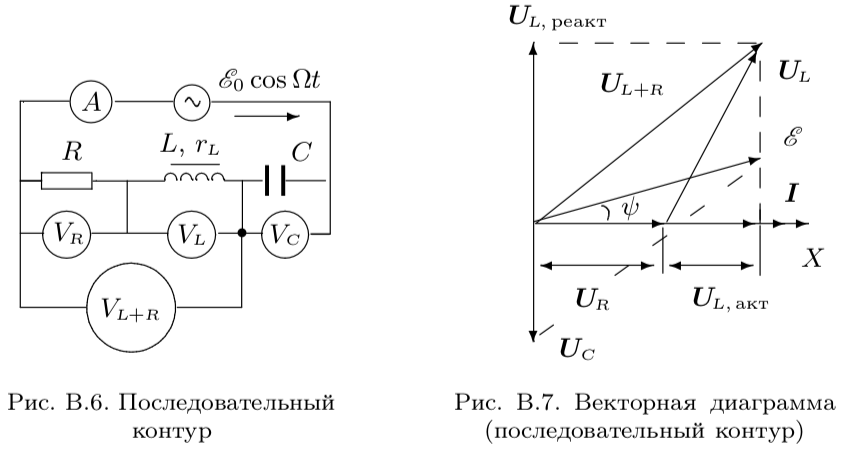
\includegraphics[width=0.9 \textwidth]{zero}\\
        	{\scriptsize
        	\begin{center}
        	\end{center}}
    	\end{center}
        \label{scheme1}
    \end{figure}
            \begin{figure}[h!]
    	\begin{center}
    		\includegraphics[width=0.9 \textwidth]{first}\\
        	{\scriptsize
        	\begin{center}
        	\end{center}}
    	\end{center}
        \label{scheme1}
    \end{figure}
            \begin{figure}[h!]
    	\begin{center}
    		\includegraphics[width=0.9 \textwidth]{sec}\\
        	{\scriptsize
        	\begin{center}
        	\end{center}}
    	\end{center}
        \label{scheme1}
    \end{figure}
\end{document}

